\chapter{Основные теоретические сведения}
RISC-V является открытым современным набором команд, который может использоваться для построения как микроконтроллеров, так и высокопроизводительных микропроцессоров. Таким образом, термин RISC-V фактически является названием для семейства различных систем команд, которые строятся вокруг базового набора команд, путем внесения в него различных расширений.

В данной работе исследуется набор команд RV32I, который включает в себя основные команды 32-битной целочисленной арифметики кроме умножения и деления. 

\section{Модель памяти}
Архитектура RV32I предполагает плоское линейное 32-х битное адресное пространство. Минимальной адресуемой единицей информации является 1 байт. Используется порядок байтов от младшего к старшему (Little Endian), то есть, младший байт 32-х битного слова находится по младшему адресу (по смещению 0). Отсутствует разделение на адресные пространства команд, данных и ввода-вывода. Распределение областей памяти между различными устройствами (ОЗУ, ПЗУ, устройства ввода-вывода) определяется реализацией.

\section{Система команд}
Большая часть команд RV32I является трехадресными, выполняющими операции над двумя заданными явно операндами, и сохраняющими результат в регистре. Операндами могут являться регистры или константы, явно заданные в коде команды. Операнды всех команд задаются явно. 

Архитектура RV32I, как и большая часть RISC-архитектур, предполагает разделение команд на команды доступа к памяти (чтение данных из памяти в регистр или запись данных из регистра в память) и команды обработки данных в регистрах.

\chapter{Индивидуальные варианты}

Данная программа выполняет найдение максимальный элемент.
Листинг \ref{lst:v1}.
\begin{lstlisting}[label=lst:v1,caption=Пример программы]
	.section .text
	.globl _start;
	len = 9 #Размер массива
	enroll = 2 #Количество обрабатываемых элементов за одну итерацию
	elem_sz = 4 #Размер одного элемента массива
	
	_start:
	la x1, _x
	addi x20, x0, (len-1)/enroll
	lw x31, 0(x1)
	addi x1, x1, elem_sz*1
	lp:
	lw x2, 0(x1)
	lw x3, 4(x1)
	bltu x2, x31, lt1
	add x31, x0, x2 #!
	lt1:    bltu x3, x31, lt2
	add x31, x0, x3
	lt2:
	add x1, x1, elem_sz*enroll
	addi x20, x20, -1
	bne x20, x0, lp
	lp2: j lp2
	
	.section .data
	_x:     .4byte 0x1
	.4byte 0x2
	.4byte 0x3
	.4byte 0x4
	.4byte 0x5
	.4byte 0x6
	.4byte 0x7
	.4byte 0x8
	.4byte 0x9
\end{lstlisting}

\clearpage

Дизассемблерный код представлен на листинге \ref{lst:v2}.

\begin{lstlisting}[label=lst:v2,caption=Дизассемблированный код примера программы]
	Disassembly of section .text:
	
	80000000 <_start>:
	80000000:       00200a13        addi    x20,x0,2
	80000004:       00000097        auipc   x1,0x0
	80000008:       03c08093        addi    x1,x1,60 # 80000040 <_x>
	
	8000000c <lp>:
	8000000c:       0000a103        lw      x2,0(x1)
	80000010:       002f8fb3        add     x31,x31,x2
	80000014:       0040a183        lw      x3,4(x1)
	80000018:       003f8fb3        add     x31,x31,x3
	8000001c:       0080a203        lw      x4,8(x1)
	80000020:       00c0a283        lw      x5,12(x1)
	80000024:       004f8fb3        add     x31,x31,x4
	80000028:       005f8fb3        add     x31,x31,x5
	8000002c:       01008093        addi    x1,x1,16
	80000030:       fffa0a13        addi    x20,x20,-1
	80000034:       fc0a1ce3        bne     x20,x0,8000000c <lp>
	80000038:       001f8f93        addi    x31,x31,1
	
	8000003c <lp2>:
	8000003c:       0000006f        jal     x0,8000003c <lp2>
\end{lstlisting}

\clearpage

Можно сказать, что данная программа эквивалентна следующему псевдокоду на языке C, представленному на листинге \ref{lst:v3}.

\begin{lstlisting}[label=lst:v3,caption=Псевдокод общей программы]
	#define len 9
	#define enroll 2
	#define elem_sz 4
	int _x[]={1,2,3,4,5,6,7,8, 9};
	void _start() {
		int x20 = len/enroll;
		int *x1 = _x;
		int x31 = x1[0];
		x1 += 1;
		do {
			int x2 = x1[0];
			int x3 = x1[1];
			if (x2 >= x31)
			x31 = x2;
			if (x3 >= x31)
			x31 = x3;
			x1 += enroll;
			x20--;
		} while(x20 != 0);
	}
\end{lstlisting}

\chapter{Результаты исследования программы}

\section{Задание №2}

На рисунке \ref{img:2} снимок экране симуляции в среде Modelsim на стадии выборки и диспетчеризации  команды с адресом 80000028 на 2-й итерации.

\begin{figure}[h]
	\centering
	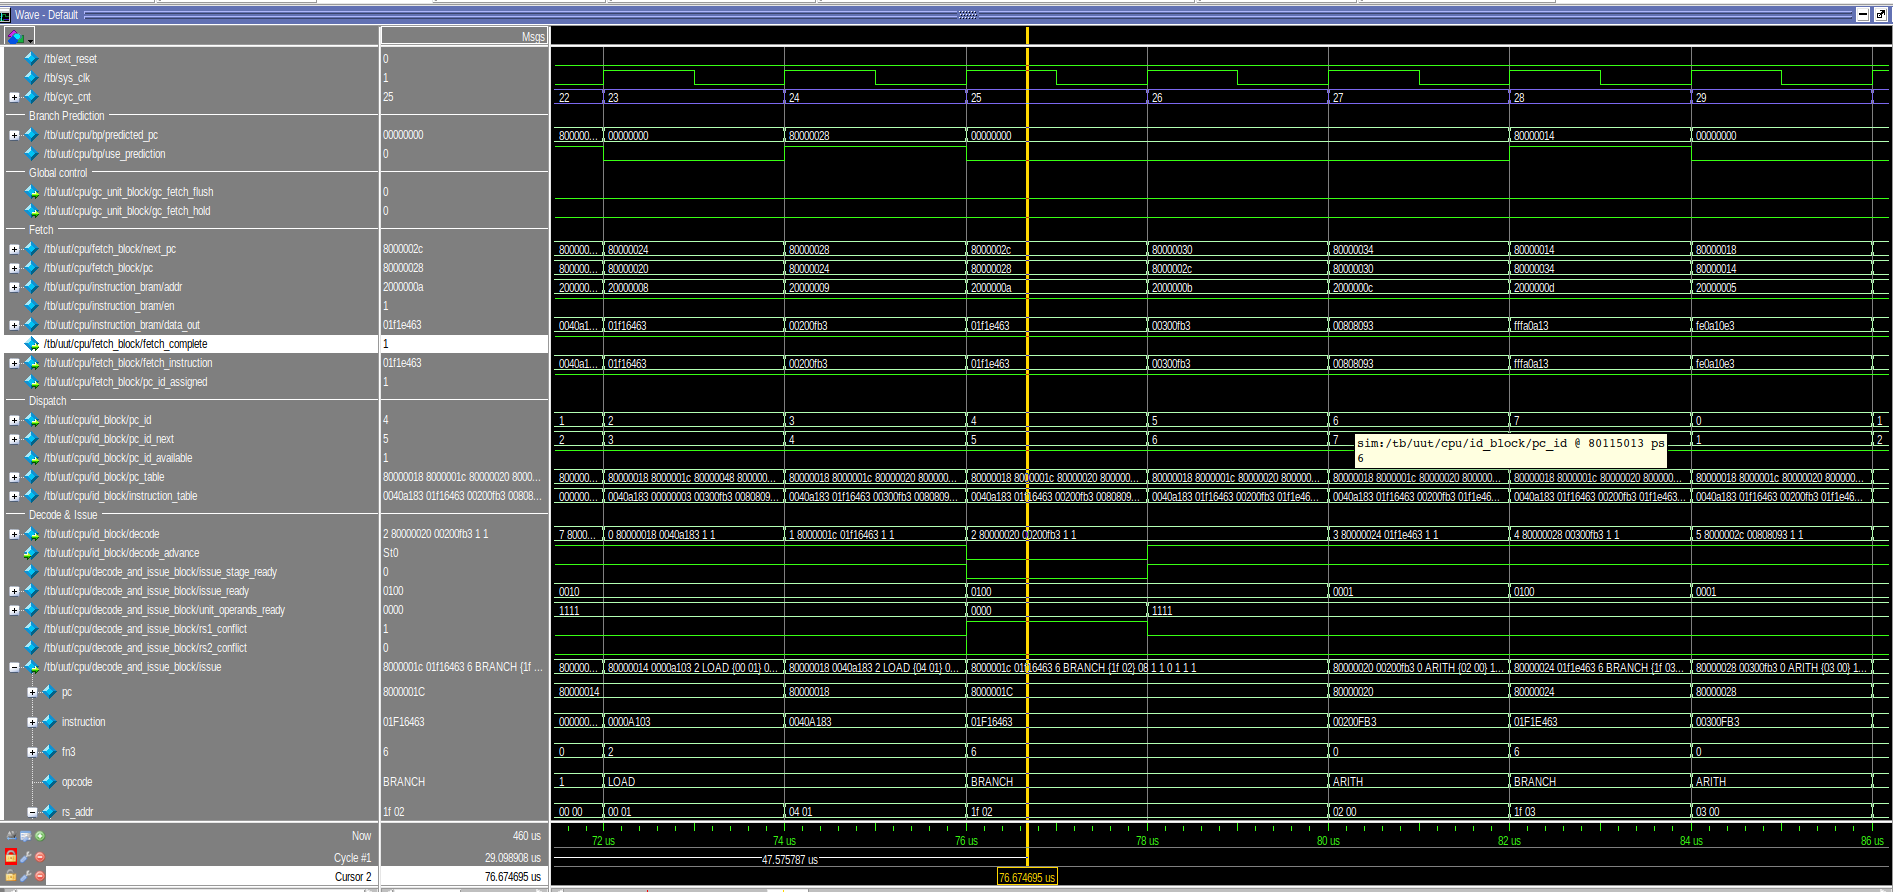
\includegraphics[height=0.35\textheight]{img/2}
	\caption{Скриншот запуска симуляция в среде Modelsim -- команды с адресом 80000028 на второй итерации.}
	\label{img:2}
\end{figure}28

\clearpage

\section{Задание №3}

\subsection*{Условие задания}
Получить снимок экрана, содержащий временную диаграмму выполнения стадии декодирования и планирования на выполнение команды с адресом 80000034 на второй итерации.

\subsection*{Результаты выполнения}

\begin{figure}[h]
	\centering
	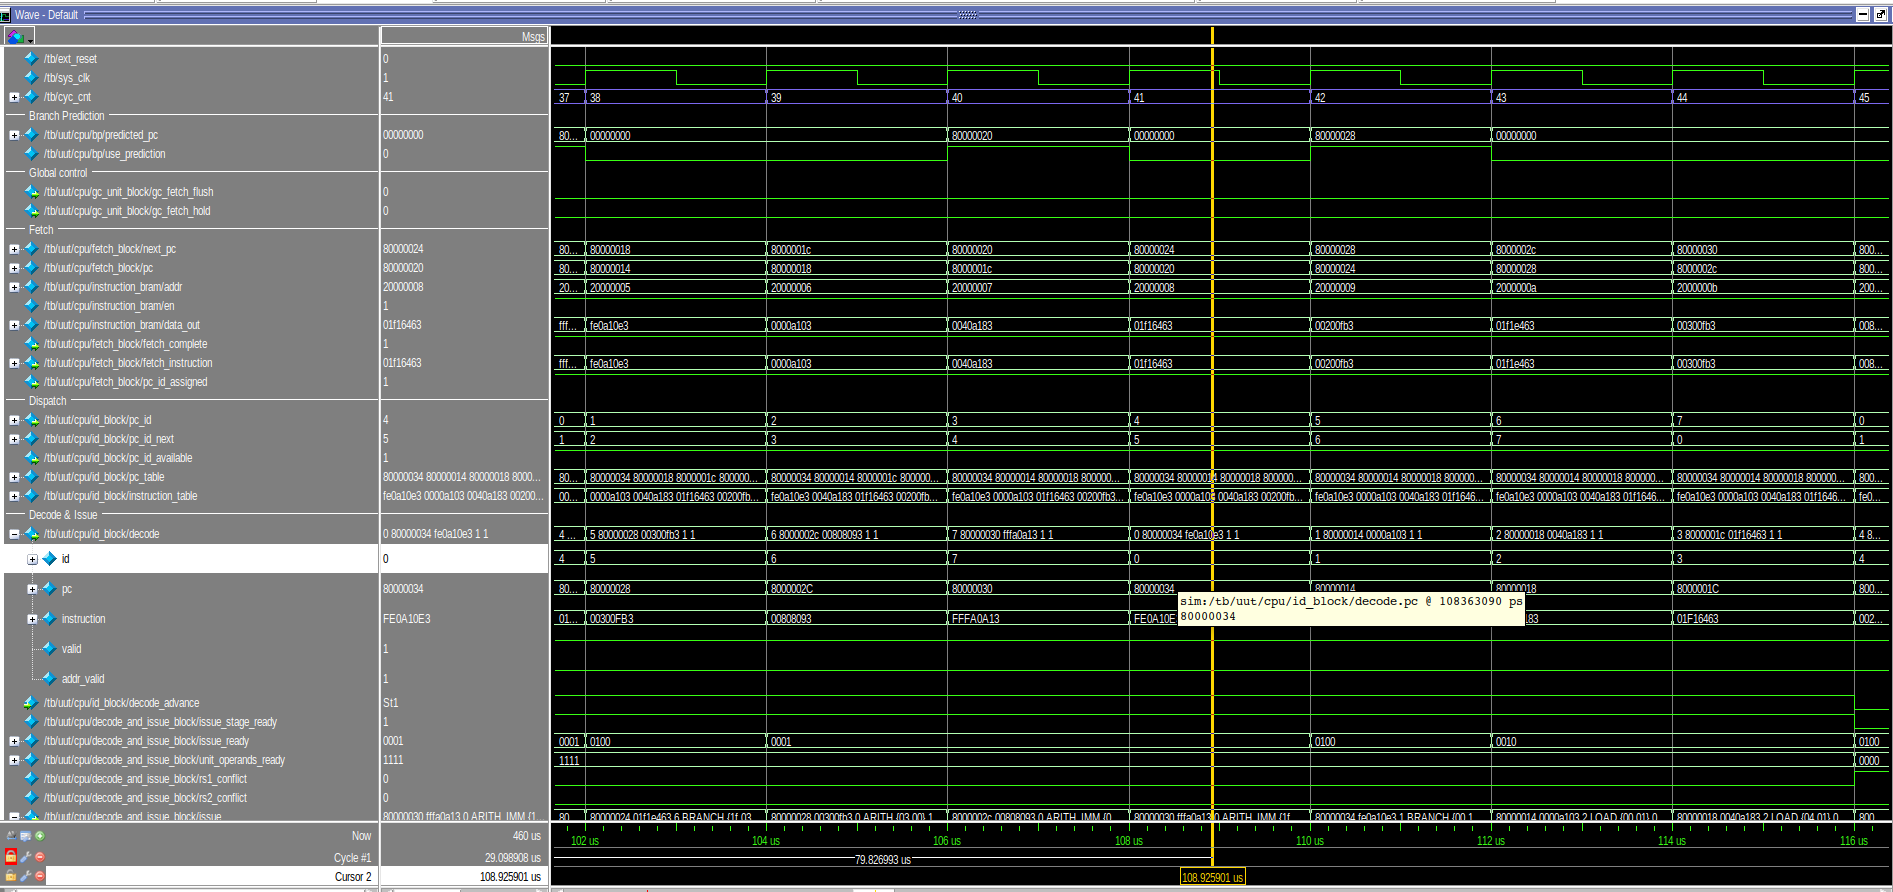
\includegraphics[height=0.35\textheight]{img/3}
	\caption{Скриншот запуска симуляция в среде Modelsim -- команды с адресом 80000034 на второй итерации.}
	\label{img:3}
\end{figure}

\section{Задание №4}

\subsection*{Условие задания}
Получить снимок экрана, содержащий временную диаграмму выполнения стадии выполнения команды с адресом 80000020 на первой итерации.

\subsection*{Результаты выполнения}

\begin{figure}[h]
	\centering
	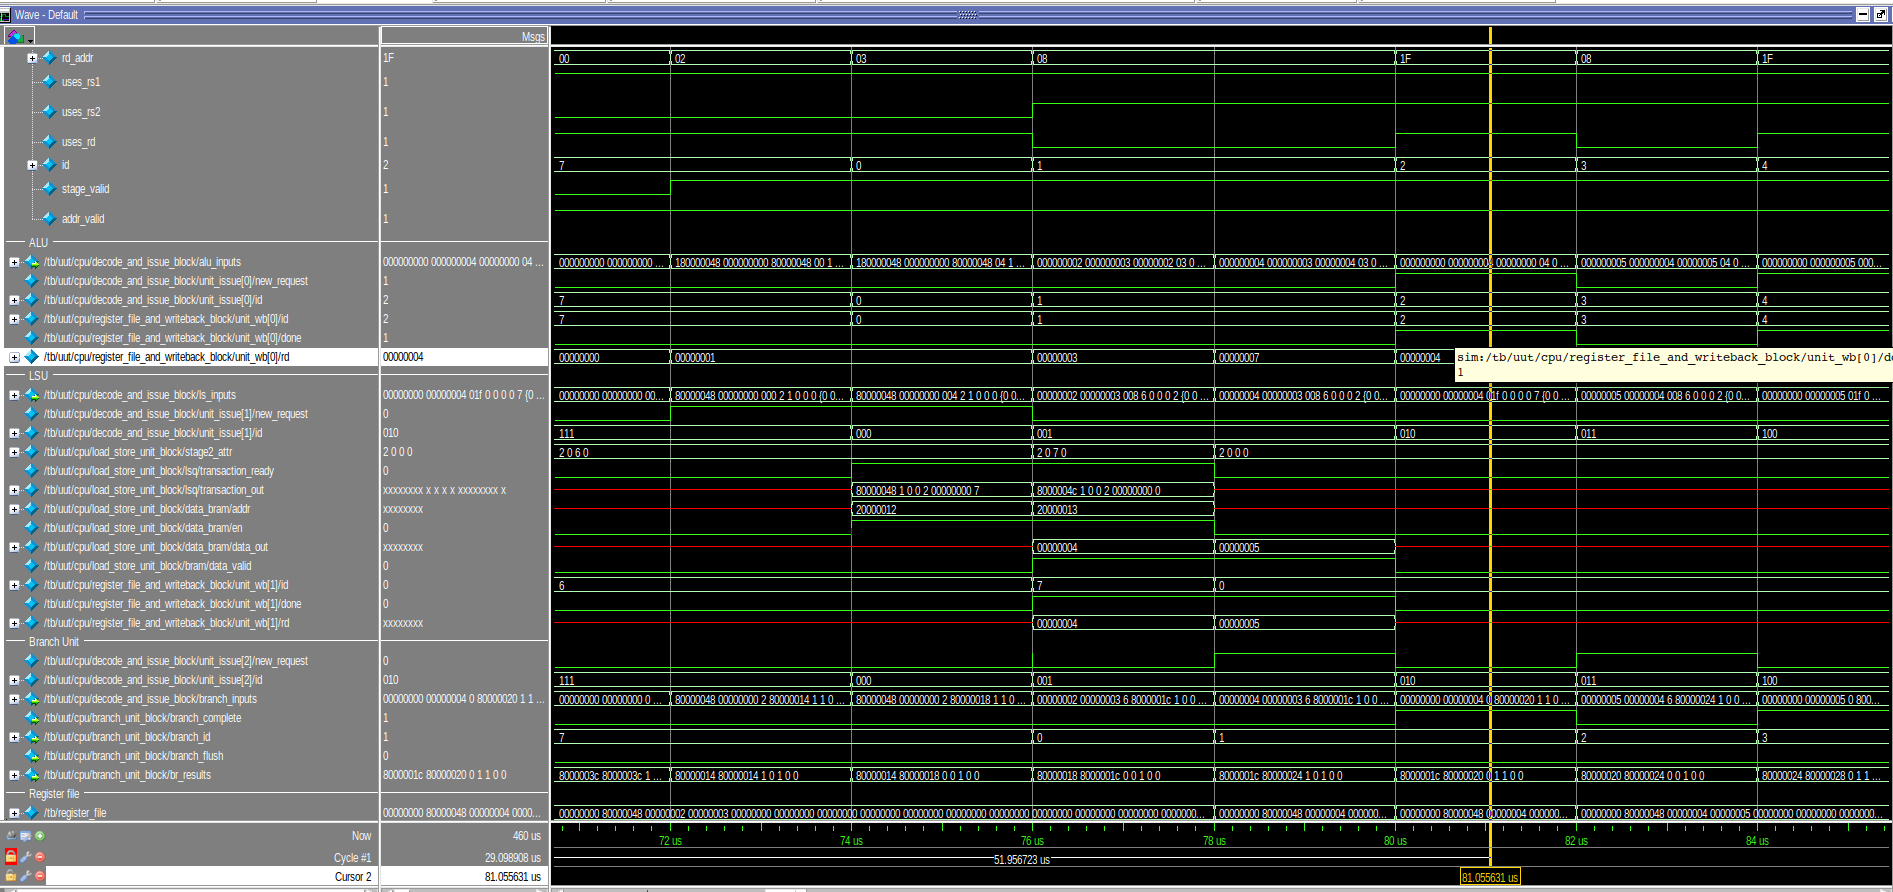
\includegraphics[height=0.35\textheight]{img/4}
	\caption{Скриншот запуска симуляция в среде Modelsim -- команды с адресом 80000020 на первой итерации.}
	\label{img:4}
\end{figure}

\section{Задание №5}

\subsubsection*{Трасса работы программы}
Трасса работы представлена на рисунке \ref{img:pipeline}.

\begin{figure}[h]
	\centering
	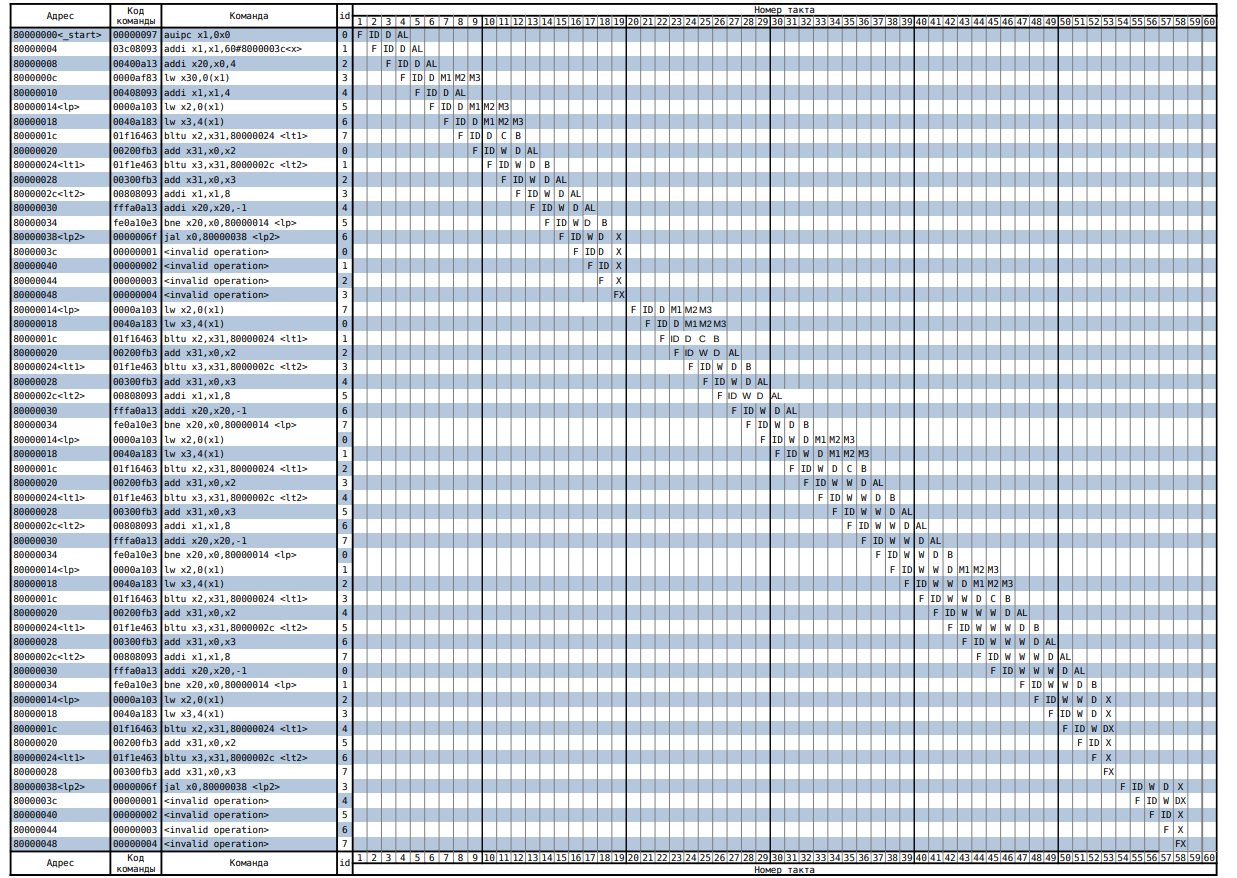
\includegraphics[height=0.5\textheight]{img/pipeline}
	\caption{Трасса работы программы.}
	\label{img:pipeline}
\end{figure}

\subsubsection*{Временные диаграммы}
Временные диаграммы сигналов, соответствующих всем стадиям выполнения команды, обозначенной в тексте программы символом \#! (add x31, x0, x2) c адресом \textit{80000020} представлены на рисунке \ref{img:fetch} -- \ref{img:alu}.

\begin{figure}[h]
	\centering
	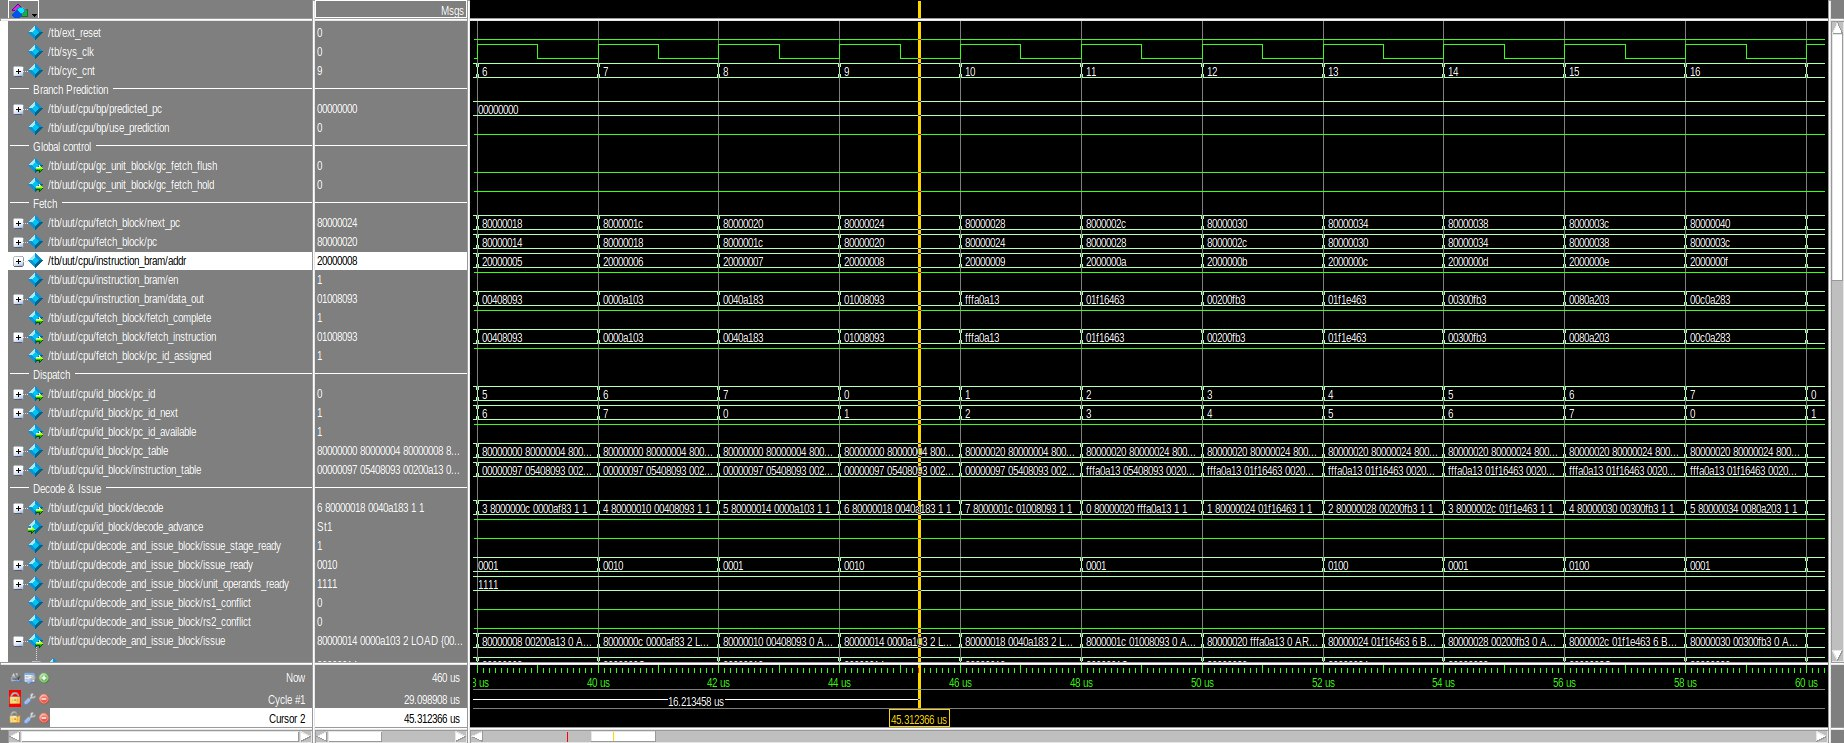
\includegraphics[height=0.3\textheight]{img/fetch}
	\caption{Временные диаграммы сигналов выборки (Fetch) с адресом 80000020.}
	\label{img:fetch}
\end{figure}

\begin{figure}[h]
	\centering
	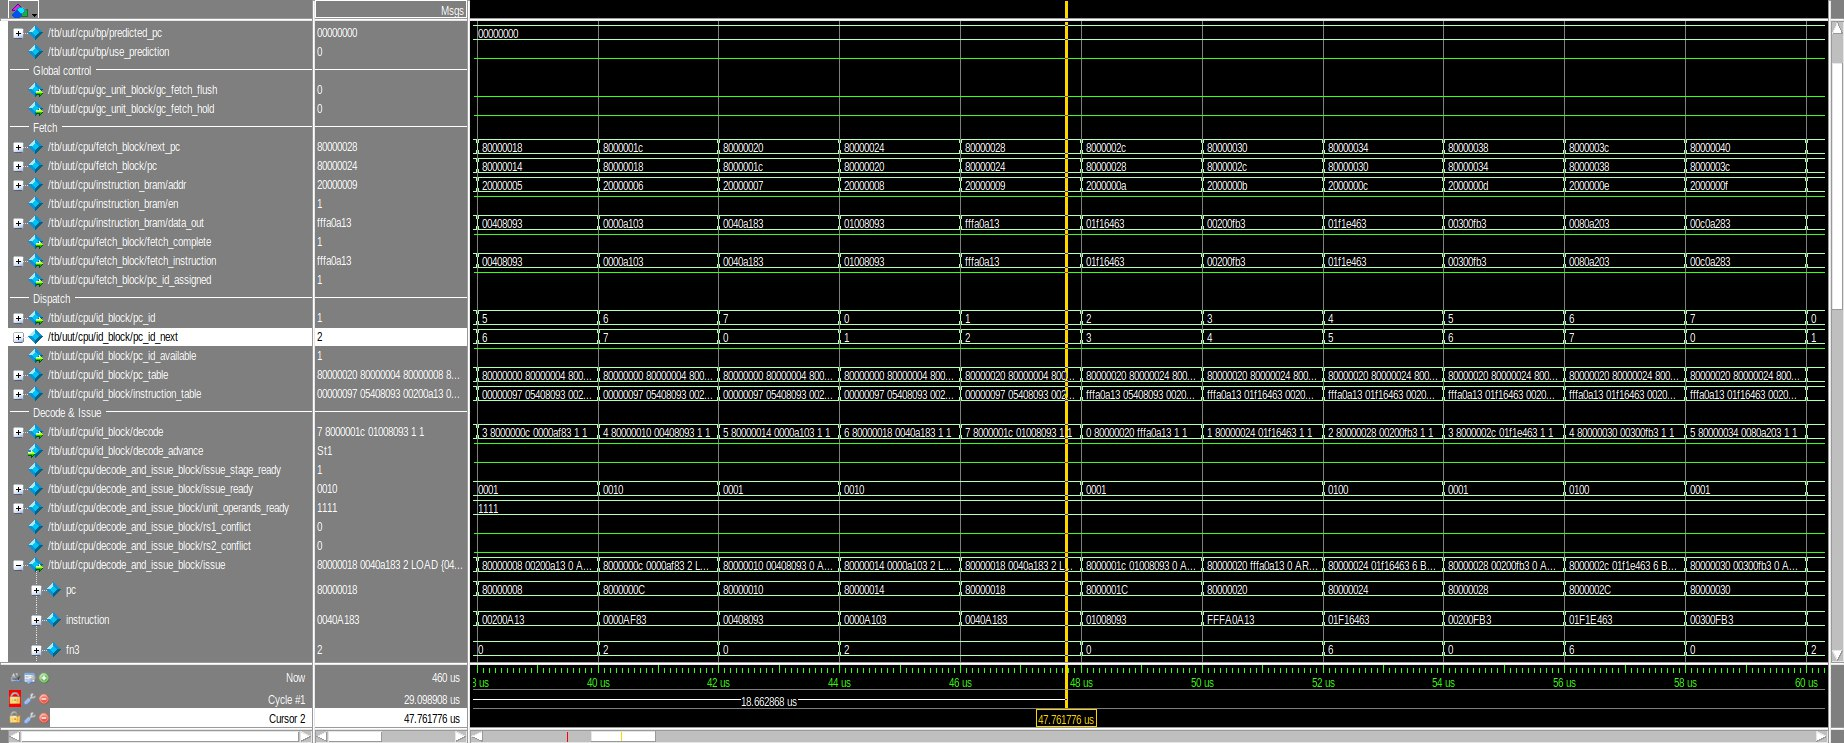
\includegraphics[height=0.3\textheight]{img/dispatch}
	\caption{Временные диаграммы сигналов диспетчеризации (Dispatch) с адресом 80000020.}
	\label{img:dispatch}
\end{figure}

\begin{figure}[h]
	\centering
	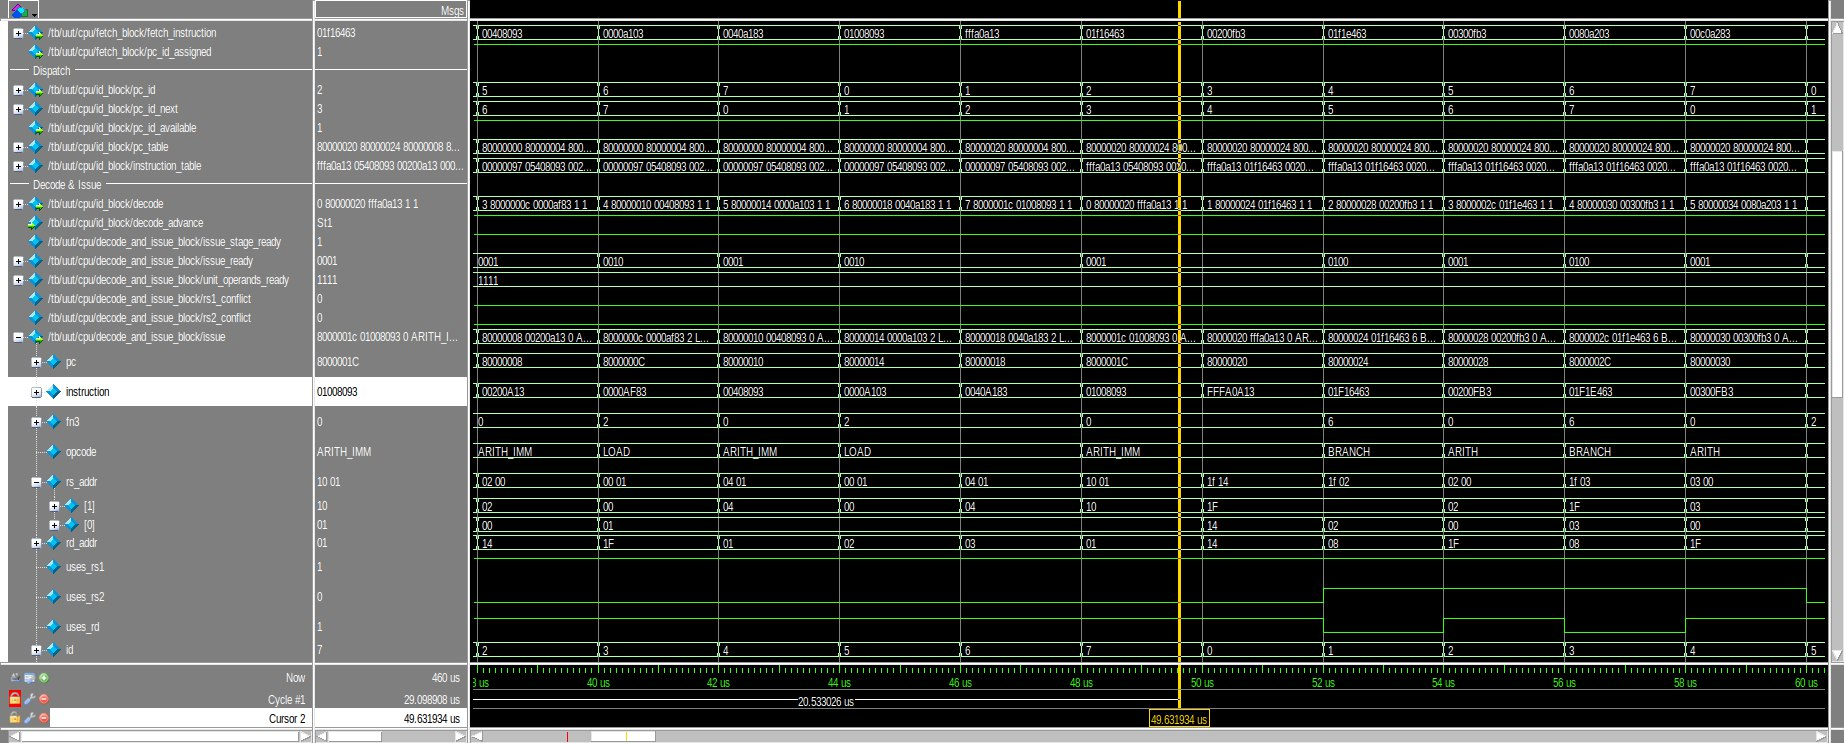
\includegraphics[height=0.3\textheight]{img/decode}
	\caption{Временные диаграммы сигналов декодирование и планирование (Decode \& Issue) с адресом 80000020.}
	\label{img:decode}
\end{figure}

\begin{figure}[h]
	\centering
	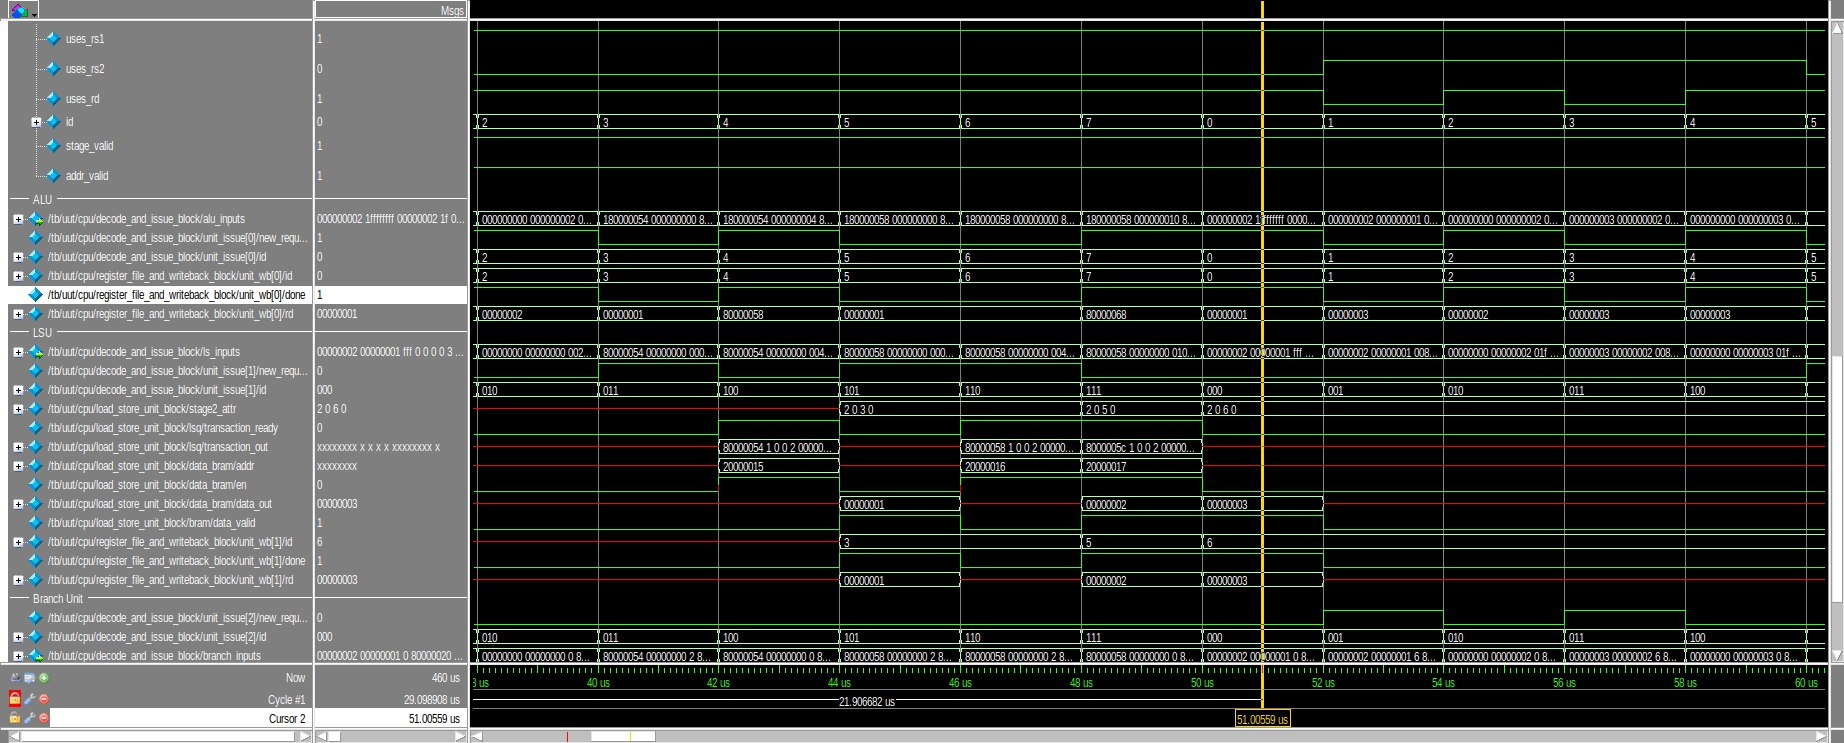
\includegraphics[height=0.3\textheight]{img/alu}
	\caption{Временные диаграммы сигналов ALU с адресом 80000020.}
	\label{img:alu}
\end{figure}

\clearpage

\subsubsection*{Вывод и предложение по оптимизации}
Как видно на трассе работы программы, представленной на рисунке, конфликты возникают из-за того, что данные загружаются в память тогда, когда уже готова выполниться операция сложения тех данных, которые загружаются. Из-за этого и возникают конфликты, так как нечего складывать, так как в памяти пока нет ничего. 

Оптимизировать программы можно тем, что сначала загрузить все данные в память, а потом их складывать. Тем самым у нас не будет конфликтов, не будет ожидания конца загрузки данных в память.

В итоге, можно будет уменьшить программу на 3 такта в оптимизированной программе.

\clearpage

\subsubsection*{Оптимизированная программа}

Код программы представлен в листинте \ref{lst:v111}

\begin{lstlisting}[label=lst:v111,caption=Код программы (оптимизированный)]
	.section .text
	.globl _start;
	len = 9 #Размер массива
	enroll = 2 #Количество обрабатываемых элементов за одну итерацию
	elem_sz = 4 #Размер одного элемента массива
	
	_start:
	la x1, _x
	addi x20, x0, (len-1)/enroll
	lw x31, 0(x1)
	addi x1, x1, elem_sz*1
	lp:
	lw x2, 0(x1)
	lw x3, 4(x1)
	addi x20, x20, -1
	bltu x2, x31, lt1
	add x31, x0, x2 #!
	lt1:    bltu x3, x31, lt2
	add x31, x0, x3
	lt2:
	add x1, x1, elem_sz*enroll
	bne x20, x0, lp
	lp2: j lp2
	
	.section .data
	_x:     .4byte 0x1
	.4byte 0x2
	.4byte 0x3
	.4byte 0x4
	.4byte 0x5
	.4byte 0x6
	.4byte 0x7
	.4byte 0x8
.4byte 0x9
\end{lstlisting}

\clearpage

Дизассемблерный код представлен на листинге \ref{lst:v222}.

\begin{lstlisting}[label=lst:v222,caption=Дизассемблированный код (оптимизированный)]
	Disassembly of section .text:
	
	80000000 <_start>:
	80000000:	00000097          	auipc	x1,0x0
	80000004:	03c08093          	addi	x1,x1,60 # 8000003c <_x>
	80000008:	00400a13          	addi	x20,x0,4
	8000000c:	0000af83          	lw	x31,0(x1)
	80000010:	00408093          	addi	x1,x1,4
	
	80000014 <lp>:
	80000014:	0000a103          	lw	x2,0(x1)
	80000018:	0040a183          	lw	x3,4(x1)
	8000001c:	fffa0a13          	addi	x20,x20,-1
	80000020:	01f16463          	bltu	x2,x31,80000028 <lt1>
	80000024:	00200fb3          	add	x31,x0,x2
	
	80000028 <lt1>:
	80000028:	01f1e463          	bltu	x3,x31,80000030 <lt2>
	8000002c:	00300fb3          	add	x31,x0,x3
	
	80000030 <lt2>:
	80000030:	00808093          	addi	x1,x1,8
	80000034:	fe0a10e3          	bne	x20,x0,80000014 <lp>
	
	80000038 <lp2>:
	80000038:	0000006f          	jal	x0,80000038 <lp2>
\end{lstlisting}
\clearpage

Можно сказать, что данная программа эквивалентна следующему псевдокоду на языке C, представленному на листинге \ref{lst:v333}.

\begin{lstlisting}[label=lst:v333,caption=Псевдокод программы (оптимизированный)]
	#define len 9
	#define enroll 2
	#define elem_sz 4
	int _x[]={1,2,3,4,5,6,7,8, 9};
	void _start() {
		int x20 = len/enroll;
		int *x1 = _x;
		int x31 = x1[0];
		x1 += 1;
		do {
			int x2 = x1[0];
			int x3 = x1[1];
			x20--;
			if (x2 >= x31)
			x31 = x2;
			if (x3 >= x31)
			x31 = x3;
			x1 += enroll;
		} while(x20 != 0);
	}
\end{lstlisting}

\clearpage

\subsubsection*{Трасса работы оптимизированной программы}
Трасса работы представлена на рисунке \ref{img:pipeline_op}.

\begin{figure}[h]
	\centering
	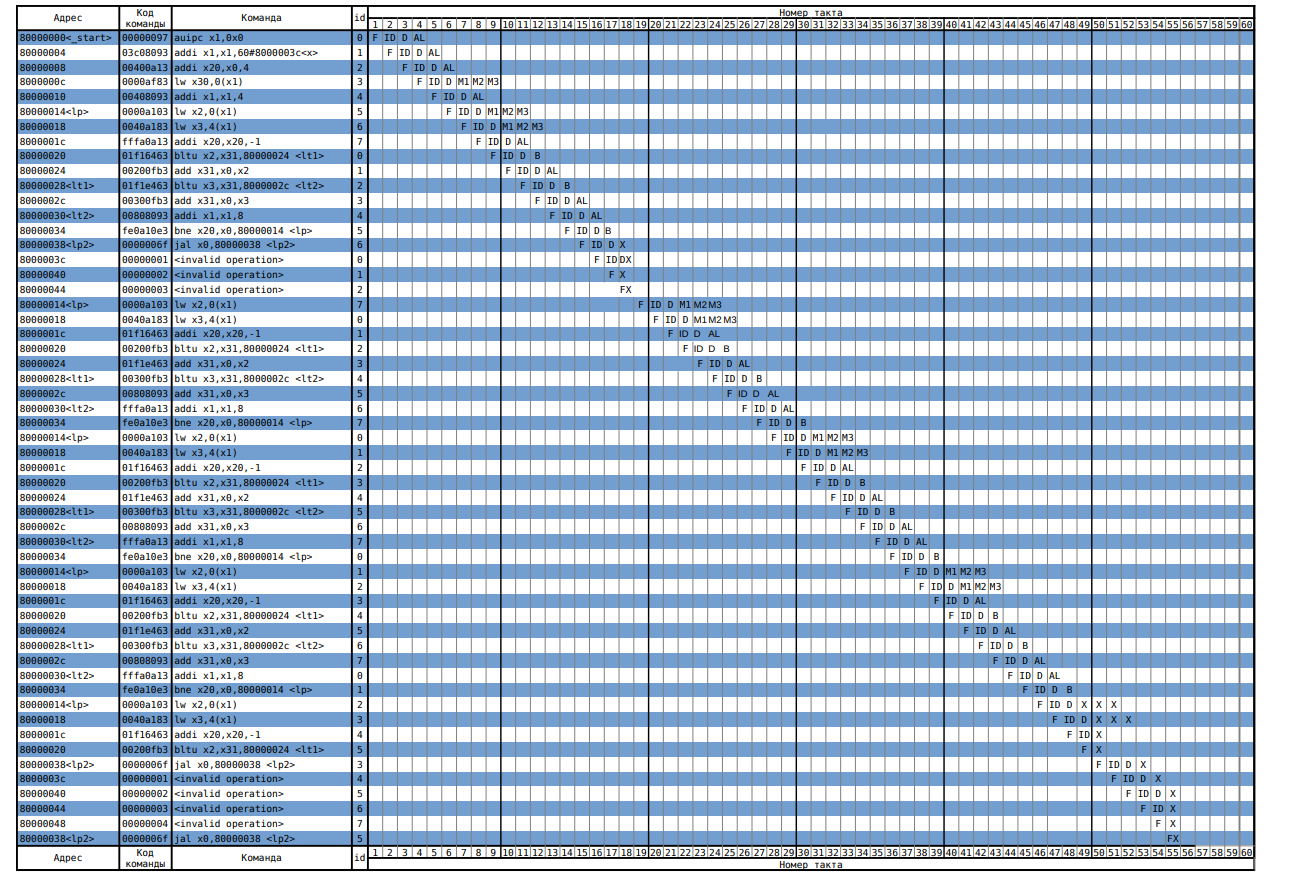
\includegraphics[height=0.48\textheight]{img/pipeline_op}
	\caption{Трасса работы оптимизированной программы.}
	\label{img:pipeline_op}
\end{figure}

